
\chapter{实验}\label{chapter_experiment}

在实验中,首先使用自动化检测工具对仿真应用进行了测试,以验证可行性和正确性。接下来对真实的应用进行了测试,收集了测试数据。

\section{仿真测试}

\subsection{仿真应用}

仿真应用(见\textbf{Listing.}\redbf{\ref{code: manifest}})应同时具有两个\textbf{公开服务}以及两个\textbf{清单声明的广播接收器}。其中每个控件之一需要人为制造内存泄漏(称为\textbf{LeakedService(Listing.\redbf{\ref{code:LeakedService}})}与\textbf{LeakedReceiver(Listing.\redbf{\ref{code:LeakedReceiver}})}),另一个则需要确保不存在内存泄漏(称为\textbf{NormalService(Listing.\redbf{\ref{code:Normal}})}与\textbf{NormalReceiver(Listing.\redbf{\ref{code:Normal}})})。
在对仿真应用进行测试时,预期的实验结果为:能够检测到\textbf{LeakedService}和\textbf{LeakedReceiver}的泄露实例,以证明该工具可以发现内存泄漏问题。而检测不到\textbf{NormalService}和\textbf{NormalReceiver}的泄露实例,以证明该工具不会将正常的组件误检。


\begin{listing}[htbp]
	\centering
	\caption{\textbf{LeakedService}主体代码}
	\begin{minted}[encoding=utf8,
	frame=single,
	framesep = 1em,
	numbers=left, 
	breaklines=true, 
	tabsize=4,
	xleftmargin=2em,xrightmargin=2em,
	fontsize=\footnotesize]{java}
public class LeakedService extends Service {
	private static final String TAG = "LeakedService";
	@Override
	public void onCreate() {
		super.onCreate();
		new Timer().scheduleAtFixedRate(new TimerTask() {
			@Override
			public void run() {
				Log.i(TAG,LeakService.this.getPackageName() + ".LeakService running ");
			}
		},1000L,3000L);
	}
}	
	\end{minted}
	\label{code:LeakedService}
\end{listing}

\begin{listing}[htbp]
	\centering
	\caption{\textbf{LeakedReceiver}主体代码}
	\begin{minted}[encoding=utf8,
	frame=single,
	framesep = 1em,
	numbers=left, 
	breaklines=true, 
	tabsize=4,
	xleftmargin=2em,xrightmargin=2em,
	fontsize=\footnotesize]{java}
public class LeakedReceiver extends BroadcastReceiver {
	private static final String TAG = "LeakedReceiver";
	private final Random random = new Random();
	@Override
	public void onReceive(Context context, Intent intent) {
		new Timer().scheduleAtFixedRate(new TimerTask() {
			@Override
			public void run() {
				Log.i(TAG,LeakReceiver.this.random.nextInt() + ".LeakReceiver running ");
			}
		},1000L,3000L);
	}
}
	\end{minted}
	\label{code:LeakedReceiver}
\end{listing}

\begin{listing}[htbp]
	\centering
	\caption{\textbf{NormalReceiver}与\textbf{NormalService}主体代码}
	\begin{minted}[encoding=utf8,
	frame=single,
	framesep = 1em,
	numbers=left, 
	breaklines=true, 
	tabsize=4,
	xleftmargin=2em,xrightmargin=2em,
	fontsize=\footnotesize]{java}
public class NormalReceiver extends BroadcastReceiver {
	private static final String TAG = "NormalReceiver";
	private final Random random = new Random();
	@Override
	public void onReceive(Context context, Intent intent) {
		Log.i(TAG,NormalReceiver.this.random.nextInt() + ".NormalReceiver running ");
		}
	}
}

public class NormalService extends Service{
	private static final String TAG = "NormalService";
		@Override
	public void onReceive(Context context, Intent intent) {
		Log.i(TAG,NormalService.this.getPackageName() + ".LeakService running ");
	}
}
	\end{minted}
	\label{code:Normal}
\end{listing}

\begin{listing}[htbp]
	\centering
	\caption{仿真应用的AndroidManifest.xml清单}
	\begin{minted}[encoding=utf8,
	frame=single,
	framesep = 1em,
	numbers=left, 
	breaklines=true, 
	tabsize=4,
	xleftmargin=2em,xrightmargin=2em,
	fontsize=\footnotesize]{xml}
<manifest
	xmlns:android="http://schemas.android.com/apk/res/android"
	xmlns:dist="http://schemas.android.com/apk/distribution"
	package="com.example.myapplication">
	<dist:module dist:instant="true" />

	<permission
		android:name="app.custom.permission"
		android:protectionLevel="signature" />
	<application ...>
		<activity android:name=".MainActivity">
			<intent-filter>
				<action android:name="android.intent.action.MAIN" />
				<category android:name="android.intent.category.LAUNCHER" />
			</intent-filter>
		</activity>
		
		<receiver
			android:name=".LeakedReceiver"
			android:exported="true">
			<intent-filter>
				<action android:name="TestActionForLeaked" />
			</intent-filter>
		</receiver>
		
		<receiver
			android:name = ".NormalReceiver"
			android:exported = "true">
			<intent-filter>
				<action android:name = "TestActionForNormal"/>
			</intent-filter>
		</receiver>
		
		<service
			android:name=".LeakedService"
			android:exported="true">
		</service>
	
		<service
			android:name = ".NormalService"
			android:exported = "true">
		</service>
	</application>
</manifest>
	\end{minted}
	\label{code: manifest}
\end{listing}

\subsection{实验结果}
实验结果(见\textbf{图.}\redbf{\ref{fig:result of mock receiver}}及\textbf{图.}\redbf{\ref{fig:result of mock service}})能正确检测到\textbf{LeakedService}和\textbf{LeakedReceiver}的内存泄漏实例,而没有误检\textbf{NormalService}以及\textbf{NormalReceiver},证明检测工具实际有效。

\begin{figure}[htbp]
	\centering
	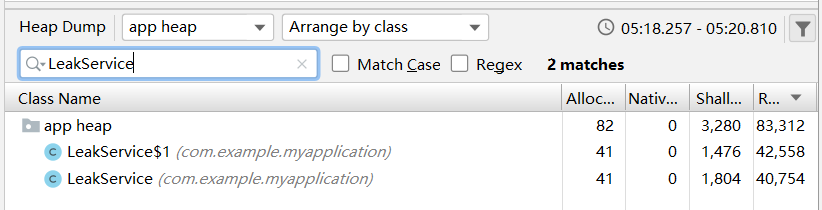
\includegraphics[width=0.9\textwidth]{service_leak_result.png} % requires the graphicx package
	\caption{检测到\textbf{LeakedService}内存泄漏实例}
	\label{fig:result of mock service}
\end{figure}
\begin{figure}[htbp]
\centering
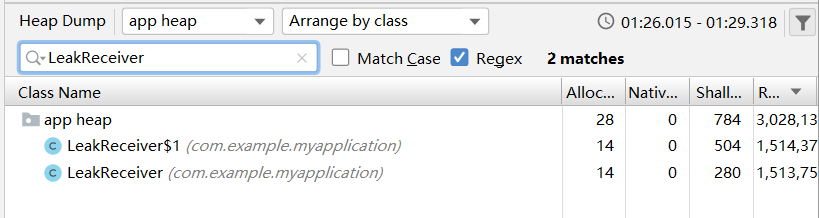
\includegraphics[width=0.9\textwidth]{receiver_leak_result.png} % requires the graphicx package
\caption{检测到\textbf{LeakedReceiver}内存泄漏实例}
\label{fig:result of mock receiver}
\end{figure}

\section{真实测试}
